\section{\scshape kNN}

\subsection{Ogólne informacje}
\begin{frame}{Ogólne informacje}
\begin{itemize}
	\item Metoda nieparametryczna.
	\item Wykorzystywany do:
	\begin{itemize}
		\item klasyfikacji;
		\item prognozowania warto"sci zmiennej losowej (regresja).
	\end{itemize}
\end{itemize}
\end{frame}

\subsection{Uczenie maszynowe}
\begin{frame}{Uczenie maszynowe}
\begin{itemize}
	\item Uczenie z przykładów (\emph{instance-based learning}).
	\item Wnioskowanie bezpo"srednio na podstawie zbioru uczącego.
	\item Złożono"sć ro"snie wraz z rozmiarem danych.
\end{itemize}
\end{frame}

\begin{frame}{Faza uczenia się}
\begin{itemize}
	\item Zbiory uczące są wektorami przestrzeni wielowymiarowej.
	\item Faza uczenia polega tylko na zapamiętaniu danych.
	\item Niski koszt.
\end{itemize}
\end{frame}

\subsection{Opis algorytmu}
\begin{frame}{Dobór parametru}
\begin{itemize}
	\item Zdefiniowanie stałej \emph{k}.
	\item \emph{k} odpowiada z liczbę analizowanych sąsiadów.
	\item Większe warto"sci redukują wypływ szumu na klasyfikację.
\end{itemize}
\end{frame}

\begin{frame}{Opis algorytmu}
\begin{itemize}
	\item Wektory zbioru uczącego posiadają etykietę.
	\item Klasyfikacja obiektu poprzez znalezienie najczę"sciej pojawiającej się etykierty w"sród \emph{k} sąsiadów.
	\begin{center}
		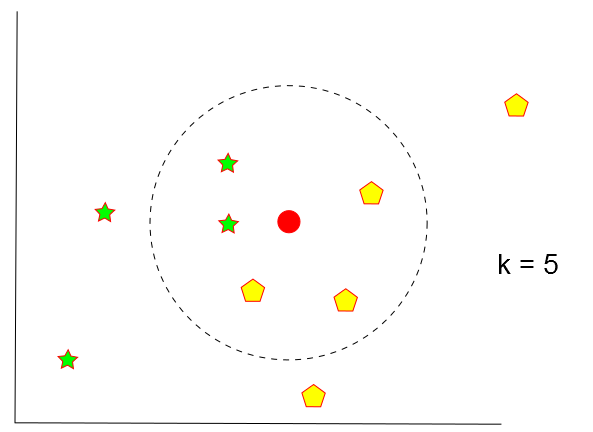
\includegraphics[keepaspectratio=true, scale=0.3]{neigh_small}
	\end{center}
	\item Odległo"sć od sąsiada okre"sla się na podstawie odpowiedniej metryki.
\end{itemize}
\end{frame}

\begin{frame}{Różne rozmiary sąsiedztw}
\begin{center}
	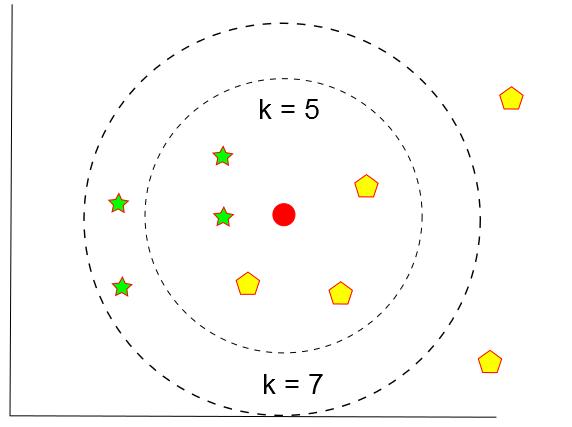
\includegraphics[keepaspectratio=true, scale=0.55]{neigh_k_small}
\end{center}
\end{frame}

\subsection{Metryki}
\begin{frame}{Własno"sci metryki ($D$)}
\begin{itemize}
	\item nieujemno"sć: $D(a,b) \ge 0$
	\item zwrotno"sć: $D(a,b) = 0 \Leftrightarrow a = b$
	\item symetria: $D(a,b) = D(b,a)$
	\item $D(a,b) + D(b,c) \ge D(a,c)$
\end{itemize}
\end{frame}

\begin{frame}{Metryka euklidesowa}
\begin{equation}
	\centering
	(a,b) = \sqrt{\sum_{i=1}^n{a_i - b_i}^2}
\end{equation}
\begin{itemize}
	\item Intuicyjna metryka (dystans między punktami).
	\item Wrażliwa na transformacje przestrzeni.
\end{itemize}
\end{frame}

\begin{frame}{Metryka Manhattan}
\begin{equation}
	\centering
	D(a,b) = \sum_{i=1}^n{|a_i - b_i|}
\end{equation}
\begin{itemize}
	\item Suma projekcji odcinków łączacych punkty na osie układu.
	\item Wrażliwa na rotację, ale nie translację.
\end{itemize}
\end{frame}

\begin{frame}{Metryka Hamminga}
\begin{itemize}
	\item Dwa ciągi znaków równej długo"sci.
	\item Liczba pozycji, na których znaki są różne
	\item {\color[rgb]{1,0,0} 5}{\color[rgb]{0,1,0} 	  23}{\color[rgb]{1,0,0} 4}{\color[rgb]{0,1,0} 1} \\
    {\color[rgb]{1,0,0} 4}{\color[rgb]{0,1,0} 23}{\color[rgb]{1,0,0} 5}{\color[rgb]{0,1,0} 1} \\
		  dystans = 2
\end{itemize}
\end{frame}

\begin{frame}{Metryka Tanimoto}
\begin{equation}
	\centering
	D(S_1,S_2) = \frac{n_1 + n_2 - 2n_12}{n_1 + n_2 - n_12}
\end{equation}
\begin{itemize}
	\item Użyteczna w taksonomii.
	\item Najlepiej działa dla takich samych lub zupełnie różnych zbiorów (bez gradacji).
\end{itemize}
\end{frame}





